This section gives you a very basic idea of how to get started with
simple tasks.  Once you have the LSST software stack installed (see
Appendix~\ref{appendix-stackinstall}), try these examples.  Remember
to source loadLSST.csh or loadLSST.sh before starting Python.  These
examples are designed to be run in interactive mode, so just type
\texttt{python} to start and copy/paste the examples in.

Python is much nicer to use interactively if you ask it to remember your command history and provide word completion; see Appendix \ref{appendix-interactivePython}.

\section{Reading and displaying a FITS image}

The main package we'll be using is the \texttt{afw} (applications
framework) package, so we start by importing some afw subpackages.
Remember to \texttt{setup afw} at your Unix prompt after sourcing
loadLSST.csh but before starting Python (see the end of
Appendix~\ref{appendix-stackinstall} if you're not sure why).

\begin{verbatim}
import lsst.afw.display.ds9 as ds9
import lsst.afw.image as afwImg

im1 = afwImg.ImageF(`image1.fits')
ds9.mtv(im1, frame=0)
\end{verbatim}

Use the name of any handy FITS image in place of image1.fits.
\texttt{ImageF} creates an image of floats, \texttt{ImageD} creates an
image of doubles.  If you do not already have ds9 running, Python will
start it for you at this point.

\section{Image arithmetic}

To save memory and time, images are operated on in-place.  That is,
you can subtract images of identical size like this:

\begin{verbatim}
import lsst.afw.display.ds9 as ds9
import lsst.afw.image as afwImg

im1 = afwImg.ImageF(`image1.fits')
im2 = afwImg.ImageF('image2.fits')

im1 -= im2
\end{verbatim}

Be careful: this modifies im1!  If you were looking to do something
like \texttt{im3=im1-im2}, where im3 is a new image, you must
explicitly force the creation of the new image and {\it then} do the
in-place arithmetic:

\begin{verbatim}
import lsst.afw.display.ds9 as ds9
import lsst.afw.image as afwImg

im1 = afwImg.ImageF(`image1.fits')
im2 = afwImg.ImageF('image2.fits')

im3 = afwImg.ImageF(im1,True)
im3 =- im2
\end{verbatim}

Again, this is because when working with large amounts of data we want
to minimize the amount of pixel copying.  The system is designed to
avoid new copies unless explicitly asked.

The first line above, beginning with im3, creates a new copy of im1, called im3.  There are
two very important things to note about this line:

\begin{itemize}

\item Setting the second argument to \texttt{True} is necessary to
  make a {\it deep copy}, meaning that the resulting image is a
  completely new image, independent of the parent image and occupying
  its own area of memory.  If the second argument is \texttt{False} or
  is omitted, a shallow copy is generated, meaning that the copy {\it
    still refers to the pixel values stored in the parent image}.
  Thus, if the pixels of a shallow copy are modified, the
  corresponding pixels in the parent image will be modified as well.
  {\it Astronomers who are new to the concept of deep and shallow
    copies will want to pay particular attention to this point.}
  Shallow copies save memory and time (for example, making postage
  stamps from a large image can be very fast and efficient) but you
  must handle them properly (don't modify the postage stamps if you
  will need to refer to the original pixel values).

\item If you are not familiar with object-oriented programming, you
  may be surprised to see that the ``function'' \texttt{ImageF}, which
  was previously called with a string (the filename) as its first and
  only argument, is now being called with {\it two} arguments, the
  first of which is not even a string.  This is a powerful
  feature. Conceptually, we know that an image can be constructed in
  many different ways.  However, many programming languages in the
  past forced us to declare different names for procedures which
  operate on different data types or take different numbers of
  arguments, even if they are conceptually similar.  With C++ and
  Python, conceptually similar operations can have the {\it same
    name}.  \texttt{ImageF} is not really a function; in
  object-oriented lingo it is a called a {\it method}.  Because it
  makes a new object, it is more specifically called a {\it
    constructor}.  We will soon see how to browse the C++
  documentation for all the different ways to construct an image.

\end{itemize}

Similar operators \texttt{+=}, \texttt{*=}, and \texttt{/=} are
defined, which do the obvious things.  The object on the right-hand
side can also be a scalar rather than an image.

\section{Cutting, copying, pasting, and writing images}

To cut out a sub-image, we must first create a \texttt{BBox} or
bounding box object, which itself must be defined by two
\texttt{PointI}\footnote{\texttt{PointI} defines a point where the
 coordinates are integers, hence the ``I''.}  objects which specify
the corners.  We then call \texttt{ImageF} in a new way:

\begin{verbatim}
import lsst.afw.image as afwImg

im1 = afwImg.ImageF(`image1.fits')

llc = afwImg.PointI(290,250)
urc = afwImg.PointI(300,260)
bbox = afwImg.BBox(llc,urc)
im4 = afwImg.ImageF(im1,bbox,False)
\end{verbatim}

\texttt{llc} and \texttt{urc} define the lower left and upper right
corners of the bounding box, respectively.  This form of the
\texttt{ImageF} constructor takes an image as its first argument, a
bounding box as its second argument, and thirdly the boolean
indicating the type of copy (\texttt{False} indicating that a deep
copy should not be made).  Shallow copies are excellent for
efficiently extracting postage stamps, as long as you remember the
implications of modifying their pixel values.

You can set pixel values using the \texttt{< <=} operator.  For
example, if you wanted to set all the pixels inside the bounding box to a
scalar value, say 99:

\begin{verbatim}
im4 < <= 99
\end{verbatim}

This also works if the right-hand side is an image of the correct size.

You can also easily mosaic images together.  The following example
makes a new mosaic image in memory and displays it.  This would be
useful for making a picture gallery of interesting galaxies, for
example.

\begin{verbatim}
import lsst.afw.display.utils as utils

im1 = afwImg.ImageF(`image1.fits')
im2 = afwImg.ImageF(`image2.fits')
im3 = afwImg.ImageF(`image3.fits')
im4 = afwImg.ImageF(`image4.fits')

images = [im1, im2, im3, im4]
labels = [`Label 1', `Label 2', `Label 3', `Label 4']

m = utils.Mosaic()
m.setMode(`square')
m.setGutter(0)

mosaic = m.makeMosaic(images)
ds9.mtv(mosaic, frame=0)
m.drawLabels(labels, frame=0)
\end{verbatim}

In the \texttt{setMode} command, the default is ``square'' which will
make the mosaic image as square as possible.  Other allowed values are
``y'' and ``x'' which make the mosaic one image wide and one image
high, respectively.  The \texttt{setGutter} command sets the number of
pixels between each image in the mosaic.

To save your mosaic image as a new FITS file:

\begin{verbatim}
afwImg.ImageF.writeFits(mosaic,'filename.fits')
\end{verbatim}


\section{Image statistics}

\texttt{math.makeStatistics} computes image statistics and returns an
object which you can then query for the statistics you want.  To save
computation time, you specify beforehand which statistics to compute,
as follows:

\begin{verbatim}
import lsst.afw.image as afwImg
import lsst.afw.math as math

im1 = afwImg.ImageF(`image1.fits')

flags = math.MEAN | math.STDEV | math.ERRORS 
stats = math.makeStatistics(im1,flags)

print stats.getResult(math.STDEV) # prints stdev AND its uncertainty
print stats.getResult(math.MEAN) # ditto for mean

\end{verbatim}

Possible statistics to calculate:
\begin{itemize}
\item ERRORS     Inlude errors of requested quantities.
\item NPOINT     number of sample points
\item MEAN     estimate sample mean
\item STDEV     estimate sample standard deviation
\item VARIANCE     estimate sample variance
\item MEDIAN     estimate sample median
\item IQRANGE     estimate sample inter-quartile range
\item MEANCLIP     estimate sample N-sigma clipped mean
\item STDEVCLIP     estimate sample N-sigma clipped stdev
\item VARIANCECLIP     estimate sample N-sigma clipped variance
\item MIN     estimate sample minimum
\item MAX     estimate sample maximum
\item SUM     find sum of pixels in the image
\item MEANSQUARE     find mean value of square of pixel values
\item NOTHING     We don't want anything.
\end{itemize}

This list is provided here to give you an idea of the capabilities in
the system, but capabilities change over time.  It's a good idea to
check the C++ documentation (as described below) for the most
up-to-date list.  The main selling point is not that you can compute
statistics---many software packages can do that---but that if you use
\texttt{maskedImage}s, the masks are {\it automatically applied} when
computing the statistics.

If you want detailed control over how the statistics are computed, for
example {\it not} using the masks, or changing the clipping from the
default 3$\sigma$ and 3 iterations, you must create a
StatisticsControl object with five arguments: the number of sigma to
clip at, the number of iterations for clipping, a specification of
which bitplanes of the mask to use (0 means use all of them; mask
bitplanes will be explained further in Chapter~\ref{chap-overview}), a
boolean indicating whether to avoid using pixels which have NaN
(not-a-number) values, and a boolean indicating whether to weight
pixels by their inverse variance.  In the example below, we use all
the default values except to ask for 5$\sigma$ rather than 3$\sigma$
clipping.

\begin{verbatim}
import lsst.afw.image as afwImg
import lsst.afw.math as math

im1 = afwImg.ImageF(`image1.fits')

flags = math.MEAN | math.STDEV | math.ERRORS 
stats = math.makeStatistics(im1,flags)

ctrl = math.StatisticsControl(5.0,3,0,True,False)
stats = math.makeStatistics(im1,flags,ctrl)
print stats.getResult(math.STDEV) 
\end{verbatim}

In this case, we get a larger STDEV because we clipped less harshly
than the default.


\section{Masked images}

So far this may seem rather mundane, but the framework has some
features that will make it much more powerful with almost no extra
work on your part.  For example, we often want to propagate
uncertainties through these arithmetic operations, and apply masks
which ensure that the operations are not done on bad areas of the
image.  The applications framework defines a \texttt{maskedImage}
which contains an image, a variance image, and a mask image.
Once you have constructed \texttt{maskedImage}s, masking and
uncertainty propagation is done {\it automatically} when you invoke
these arithmetic operations.

A couple caveats first, before the examples:
\begin{itemize}
\item The mask part of MaskedImage is not just another image but
is created with MaskU, where the ``U'' stands for ``unsigned''.
\item The error message you get when you use a constructor
incorrectly is not very specific.  You might get a list of all
possible constructors, which is not very helpful when there
are dozens and you just want to know where your one little mistake
is.  (Not that the software COULD know what you mean, of course,
but it's different from say, C, where the compiler knows what type
the third argument should be, and tells you quite specifically when you
give it the wrong type.)
\end{itemize}

To create a masked image from nothing, use the following example, substituting your own dimensions for the ones included here.

\begin{verbatim}
import lsst.afw.image as afwImg

a = afwImg.ImageF(10,10) # image
v = afwImg.ImageF(a.getDimensions()) # variance image
m = afwImg.MaskU(a.getDimensions()) # mask
mi = afwImg.MaskedImageF(a,m,v) # put it all together into one maskedImage
\end{verbatim}

That last line is a bit of a bore as you have to remember the \verb|F|;  fortunately you can get the computer to do the work by saying
\begin{verbatim}
mi2 = afwImg.makeMaskedImage(a, m, v)
\end{verbatim}

Alternatively, you can create a masked image and then tell Python to get the components.  In the following example, we generate a masked image of size 100 x 100 pixels, set all of the pixels in the variance image to 1.0, and set all of the pixels in the base (??) image to 32.0.  Then, we assign the ``saturated'' mask plane to the mask, and to make things a bit more interesting, we apply the mask to pixels (50,50) and (60,60).  

\begin{verbatim}
import lsst.afw.image as afwImg
import lsst.afw.display.ds9 as ds9

mi = afwImg.MaskedImageF(100,100)

vari = mi.getVariance()
vari.set(1.0)

img = mi.getImage()
img.set(32.0)

mask = mi.getMask()

bitMask = mask.getPlaneBitMask('SAT')
mask.set(50,50,bitMask)
mask.set(60,60,bitMask)

ds9.mtv(mi)
\end{verbatim}

You can use the methods in the ``Image Statistics'' section to verify that you have indeed masked those 2 pixels:

\begin{verbatim}
import lsst.afw.image as afwImg
import lsst.afw.display.ds9 as ds9
import lsst.afw.math as math

mi = afwImg.MaskedImageF(100,100)
vari = mi.getVariance().set(1.0)
mask = mi.getMask()
img = mi.getImage()
img.set(32)

stats = math.makeStatistics(mi,math.NPOINT)
print stats.getValue(math.NPOINT)
\end{verbatim}

(Note: You can leave off ``print'' if you are running this interactively.)  Notice that this prints out the value 10000, which is the number of pixels in our images.

\begin{verbatim}
bitMask = mask.getPlaneBitMask('SAT')
mask.set(50,50,bitMask)
mask.set(60,60,bitMask)

ctrl = math.StatisticsControl()
ctrl.setAndMask(bitMask)
stats = math.makeStatistics(mi,math.NPOINT,ctrl).getValue()
\end{verbatim}

Now, the value printed is 9998, which is perfect because we masked 2 pixels.  And we avoided typing \verb|math.NPOINT| twice (which only works if you're asking for one thing).

\section{Exposures}
As you have probably already noticed, calling an object an ``image'' in the LSST environment is not as simple as it sounds - there are several classes which a layperson would consider images, but an astronomer using the LSST software must know the difference.

To begin, an ``image'' is simply a 2D array of pixels.

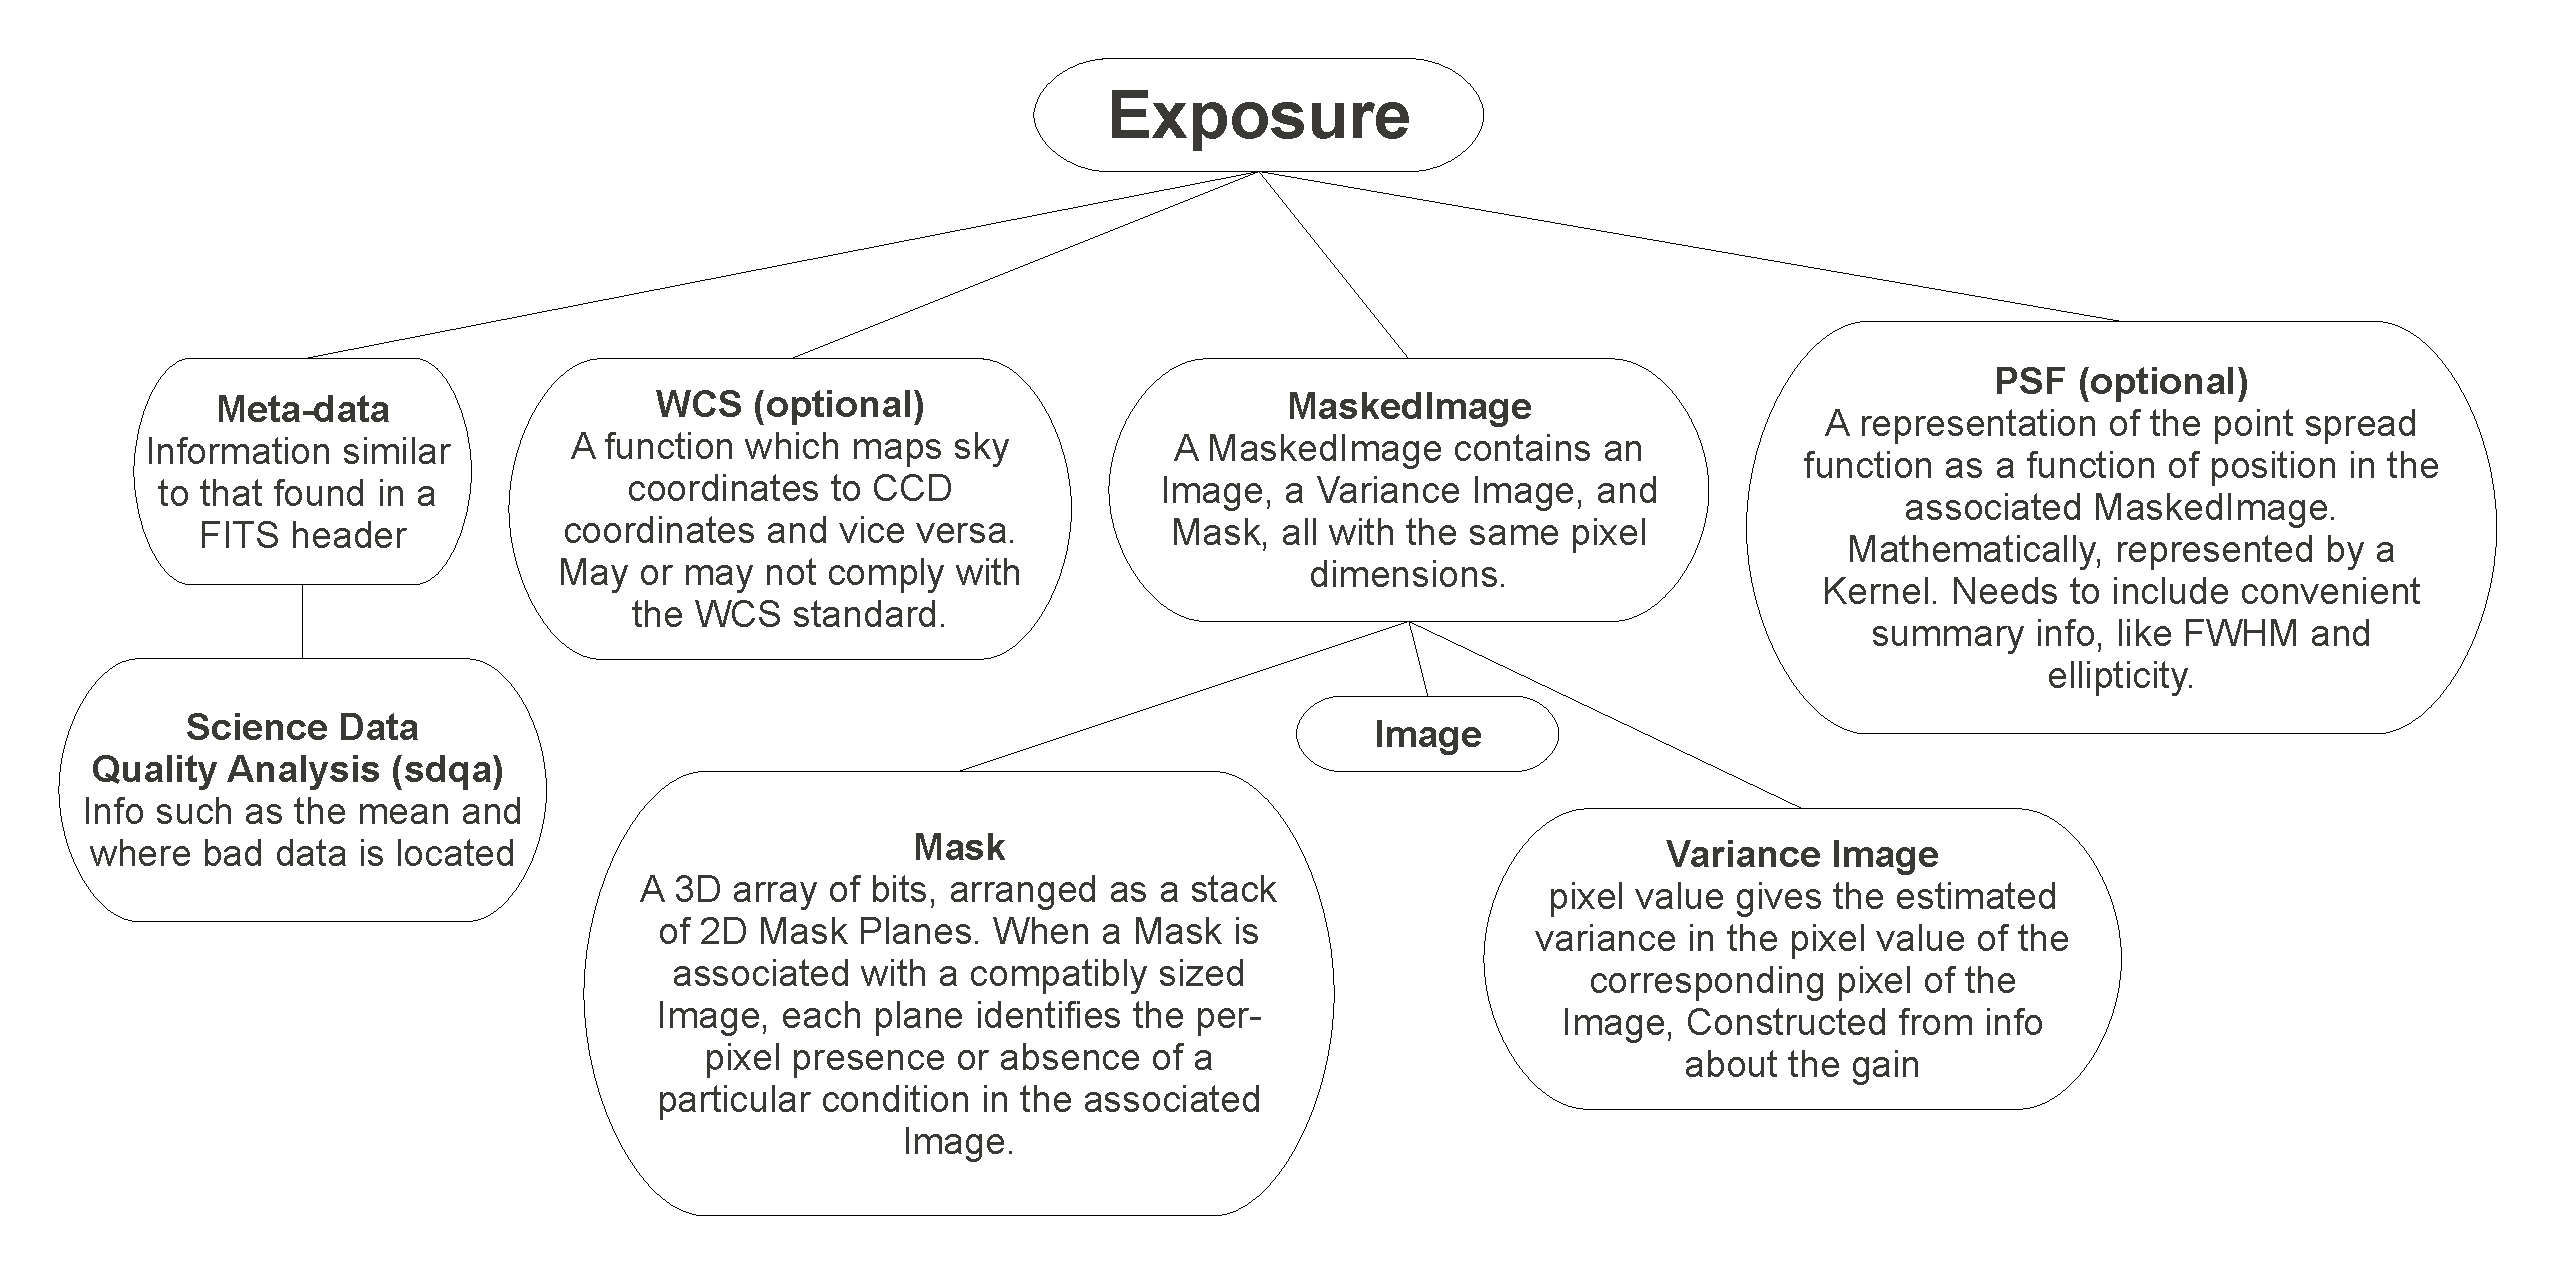
\includegraphics[angle=90,scale=0.5]{./figures/exposure.pdf}
%Not sure what to do with this, so it's on its side for now.



%See also the ``How to display an image'' link on the ``Related Pages''
%tab of the aforementioned documentation, for additional image
%commands.

\vskip0.5in

This concludes our set of ``Hello, world'' examples.  To move beyond
these very simple tasks, we must first get an overview of what's
available in the LSST packages.
